\section{Navigation}

Navigation is a basic task for Duckieboat, user can tap the destination on PC, while Duckieboat received data from PC through wifi, it will control it to where user demands.

\subsection{Localization}
We can get current position and orientation of Duckieboat from GPS and IMU. After we choose a destination(G), data output from both sensors will go through Kalman filter before entering the compute units. 

\subsection{Algorithm}
The distance(D) and angle(A) between boat and destination will be calculated, each result will go through a PID controller and send it to motor controllers to navigate Duckieboat to our desire destination.

\begin{figure}[h]
	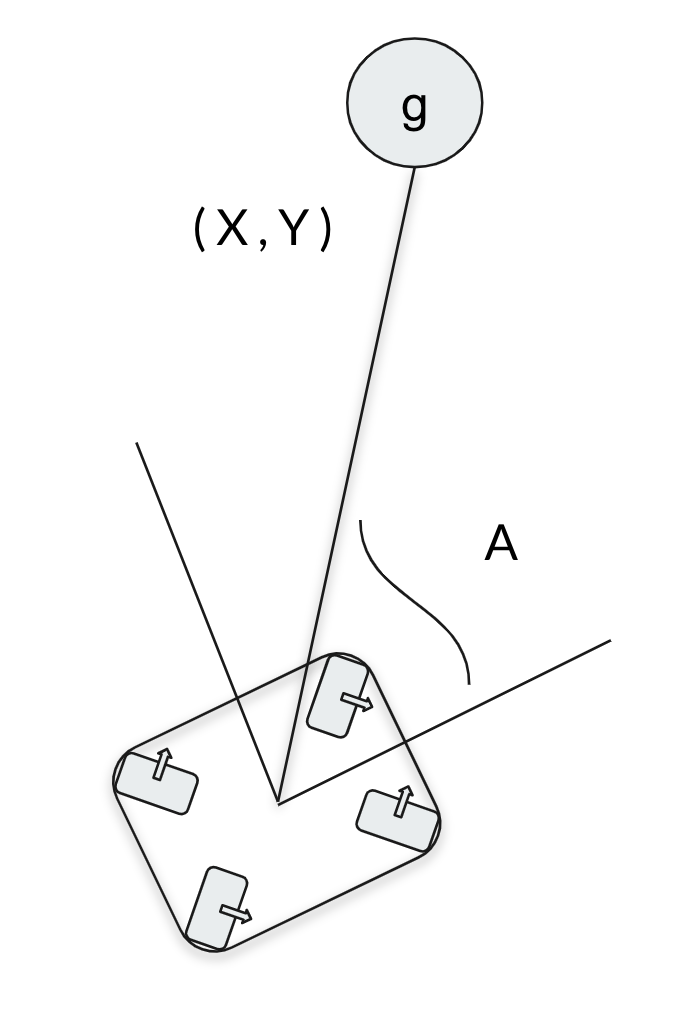
\includegraphics[width=0.5\columnwidth]{images/navigation.png}
	\centering
	\caption{navigation parameter}
	\label{figure:navigation}
\end{figure}

The frequency of data output from GPS and IMU is 10 Hz. Hence, we made Duckieboat enter station keeping mode after the distance is below 5 meters.

